\section{Perspektywa logiczna}

\subsection{Diagram klas}

\begin{figure}[H]
    \centering
    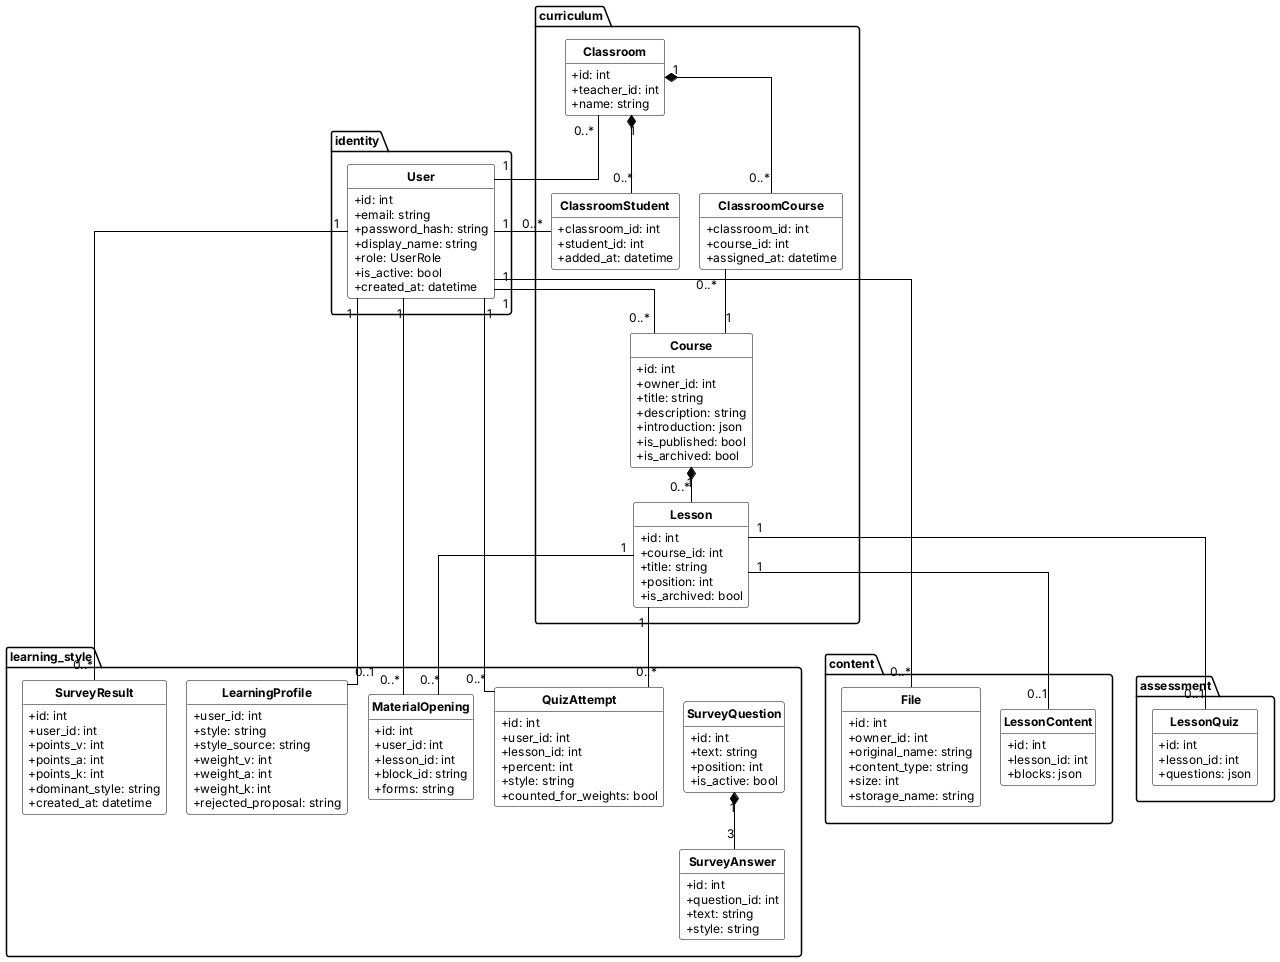
\includegraphics[width=\textwidth]{images/classes.png}
    \caption{Diagram klas (klasy pogrupowane według modułów systemu)}
    \label{fig:classes}
\end{figure}

\subsection{Uporządkowany alfabetycznie wykaz klas}

\textbf{Classroom} -- klasa (grupa uczniów) prowadzona przez jednego nauczyciela. \\
\textit{Atrybuty:} \texttt{id}, \texttt{teacher\_id}, \texttt{name}.

\vspace{0.5em}
\textbf{ClassroomCourse} -- przypisanie kursu do klasy; uczniowie klasy widzą przypisany kurs, także prywatny. \\
\textit{Atrybuty:} \texttt{classroom\_id}, \texttt{course\_id}, \texttt{assigned\_at}.

\vspace{0.5em}
\textbf{ClassroomStudent} -- przynależność ucznia do klasy. \\
\textit{Atrybuty:} \texttt{classroom\_id}, \texttt{student\_id}, \texttt{added\_at}.

\vspace{0.5em}
\textbf{Course} -- kurs nauczyciela: opis widoczny w katalogu, wstęp i lista lekcji. Kurs jest prywatny albo opublikowany; usunięcie oznacza archiwizację. \\
\textit{Atrybuty:} \texttt{id}, \texttt{owner\_id}, \texttt{title}, \texttt{description}, \texttt{introduction} (dokument edytora), \texttt{is\_published}, \texttt{is\_archived}.

\vspace{0.5em}
\textbf{File} -- plik wgrany przez nauczyciela (obraz, nagranie, film, PDF), przechowywany na dysku pod losową nazwą. \\
\textit{Atrybuty:} \texttt{id}, \texttt{owner\_id}, \texttt{original\_name}, \texttt{content\_type}, \texttt{size}, \texttt{storage\_name}.

\vspace{0.5em}
\textbf{LearningProfile} -- profil ucznia: aktualny styl (np. \texttt{V}, \texttt{VA}), źródło stylu (ankieta, wybór ręczny, adaptacja), wagi form V, A, K (0--30) oraz odrzucona propozycja zmiany stylu. \\
\textit{Atrybuty:} \texttt{user\_id}, \texttt{style}, \texttt{style\_source}, \texttt{weight\_v}, \texttt{weight\_a}, \texttt{weight\_k}, \texttt{rejected\_proposal}.

\vspace{0.5em}
\textbf{Lesson} -- lekcja kursu w kolejności ustalonej przez nauczyciela. \\
\textit{Atrybuty:} \texttt{id}, \texttt{course\_id}, \texttt{title}, \texttt{position}, \texttt{is\_archived}.

\vspace{0.5em}
\textbf{LessonContent} -- treść lekcji jako uporządkowana lista bloków: tekstu oraz załączników z formami V/A/K. \\
\textit{Atrybuty:} \texttt{id}, \texttt{lesson\_id}, \texttt{blocks} (JSON).

\vspace{0.5em}
\textbf{LessonQuiz} -- quiz na końcu lekcji: do 20 pytań jednokrotnego wyboru, każde wspólne albo dotyczące materiału formy V, A lub K. \\
\textit{Atrybuty:} \texttt{id}, \texttt{lesson\_id}, \texttt{questions} (JSON).

\vspace{0.5em}
\textbf{MaterialOpening} -- zapis pierwszego rozwinięcia zwiniętego materiału przez ucznia; jego formy wchodzą do stylu efektywnego lekcji. \\
\textit{Atrybuty:} \texttt{id}, \texttt{user\_id}, \texttt{lesson\_id}, \texttt{block\_id}, \texttt{forms}.

\vspace{0.5em}
\textbf{QuizAttempt} -- podejście ucznia do quizu: wynik w procentach, styl efektywny w chwili podejścia i informacja, czy podejście zmieniło wagi. \\
\textit{Atrybuty:} \texttt{id}, \texttt{user\_id}, \texttt{lesson\_id}, \texttt{percent}, \texttt{style}, \texttt{counted\_for\_weights}.

\vspace{0.5em}
\textbf{SurveyAnswer} -- odpowiedź na pytanie ankiety, przypisana do jednej formy V, A lub K. \\
\textit{Atrybuty:} \texttt{id}, \texttt{question\_id}, \texttt{text}, \texttt{style}.

\vspace{0.5em}
\textbf{SurveyQuestion} -- pytanie ankiety VAK (20 pytań, po 3 odpowiedzi). \\
\textit{Atrybuty:} \texttt{id}, \texttt{text}, \texttt{position}, \texttt{is\_active}.

\vspace{0.5em}
\textbf{SurveyResult} -- wynik jednego wypełnienia ankiety (historia wyników). \\
\textit{Atrybuty:} \texttt{id}, \texttt{user\_id}, \texttt{points\_v}, \texttt{points\_a}, \texttt{points\_k}, \texttt{dominant\_style}, \texttt{created\_at}.

\vspace{0.5em}
\textbf{User} -- konto użytkownika z rolą ucznia, nauczyciela albo administratora. Konto można zablokować. \\
\textit{Atrybuty:} \texttt{id}, \texttt{email}, \texttt{password\_hash}, \texttt{display\_name}, \texttt{role}, \texttt{is\_active}, \texttt{created\_at}.

\subsection{Model danych}

Baza danych PostgreSQL zawiera 15 tabel odpowiadających klasom z diagramu. Najważniejsze relacje:

\begin{itemize}[leftmargin=*]
    \item \texttt{users} 1:N \texttt{courses} (autor), 1:N \texttt{classrooms} (nauczyciel), 1:1 \texttt{learning\_profiles}, 1:N \texttt{survey\_results}, \texttt{quiz\_attempts}, \texttt{material\_openings}
    \item \texttt{courses} 1:N \texttt{lessons}; \texttt{lessons} 1:1 \texttt{lesson\_contents} i \texttt{lesson\_quizzes}
    \item \texttt{classrooms} N:M \texttt{users} (przez \texttt{classroom\_students}) oraz N:M \texttt{courses} (przez \texttt{classroom\_courses}); usunięcie klasy usuwa tylko powiązania
\end{itemize}

\subsection{Reguły adaptacji}

Mechanizm adaptacji to zbiór reguł zapisanych jako czyste funkcje (bez bazy danych i bez frameworka), dzięki czemu są przewidywalne, wyjaśnialne i pokryte testami. Nie wymagają danych treningowych ani zewnętrznego modelu AI.

\subsubsection{Styl i wagi z ankiety}
Każda odpowiedź ankiety daje punkt jednej formie. Styl ucznia to forma z największą liczbą punktów; przy remisie styl jest mieszany (np. \texttt{VA}). Wagi startowe V, A, K są równe punktom z ankiety.

\subsubsection{Podanie lekcji}
Bloki są wyświetlane w kolejności nauczyciela, tekst zawsze. Załącznik, którego żadna forma nie należy do stylu ucznia, jest \textbf{zwinięty w miejscu} -- uczeń widzi, że materiał istnieje, i może go rozwinąć. Nad lekcją system pokazuje uzasadnienie, np. ,,\ldots bo tak wyszło w ankiecie (V 9 / A 8 / K 3)''.

\subsubsection{Styl efektywny lekcji}
Styl efektywny to styl ucznia uzupełniony o formy materiałów, które uczeń rozwinął w danej lekcji. Od niego zależą pytania quizu (uczeń dostaje pytania wspólne i pytania o materiały form, z których korzystał) oraz to, które wagi zmienia wynik.

\subsubsection{Aktualizacja wag po quizie}
\begin{itemize}[leftmargin=*]
    \item Wynik co najmniej 70\% oznacza zaliczenie
    \item Każda litera stylu efektywnego dostaje $+1$ przy zaliczeniu albo $-1$ przy niezaliczeniu (zakres wag 0--30)
    \item W danej lekcji liczy się tylko pierwsze zaliczenie i pierwsze niezaliczenie -- kolejne podejścia nie zmieniają wag, więc nie da się ich ,,nabić''
\end{itemize}

\subsubsection{Propozycja zmiany stylu}
System proponuje zmianę stylu, gdy jedna forma ma samodzielnie najwyższą wagę (bez remisu) i nie należy do stylu ucznia. Uczeń przyjmuje propozycję albo ją odrzuca -- odrzucona propozycja nie wraca. Styl wybrany ręcznie wyłącza propozycje, a ponowna ankieta ustawia styl i wagi od nowa.

\subsubsection{Przykład}
Uczeń w ankiecie uzyskał V 9 / A 8 / K 3, więc jego styl to V. Uczy się z materiałów wzrokowych i rozwiązuje quizy w czterech lekcjach:

\begin{table}[H]
\centering
\begin{tabular}{|l|c|c|c|}
\hline
\textbf{Zdarzenie} & \textbf{Wynik} & \textbf{Zmiana} & \textbf{Wagi V / A / K} \\ \hline
Ankieta & -- & -- & 9 / 8 / 3 \\ \hline
Quiz w lekcji 1 & 85\% & V $+1$ & 10 / 8 / 3 \\ \hline
Quiz w lekcji 2 & 55\% & V $-1$ & 9 / 8 / 3 \\ \hline
Quiz w lekcji 3 & 40\% & V $-1$ & 8 / 8 / 3 \\ \hline
Quiz w lekcji 4 & 45\% & V $-1$ & 7 / 8 / 3 \\ \hline
\end{tabular}
\caption{Zmiana wag ucznia o stylu V}
\end{table}

Po czwartym quizie forma A jest jedynym liderem wag i nie należy do stylu ucznia, więc system wyświetla propozycję: ,,Wagi wskazują na materiały słuchowe -- przełączyć?'' z uzasadnieniem ,,Wagi stylów po quizach: V 7 / A 8 / K 3''.